\chapter{Experimantal Setup}
\label{ch:ExSetup}

Chapter \ref{ch:PotenHWSetup} discussed the possible options to implement a MIMO setup. The first option (section \ref{sec:USRP}) was not viable due to technical limitations as it is described in Appendix \ref{sec:USRPSync}.

The second option (section \ref{sec:MIMOAFW}) was financially unfeasible as the additional hardware for the modular MIMO set was to cost over €80.000.

The only viable option was to use the LTE AFW with a MIMO Extension, although limited to a 2x2 MIMO system, was sufficient in this case.

\section{LTE Application Framework MIMO Extension}\label{sec:LTEAFWMIMOExt}

LTE AFW is a SISO LTE Release 10 implementation, where as LTE AFW 2x2 MIMO Extension was developed internally by NI as a plugin to the SISO framework. This software is not readily available for customers to purchase, but it was given to MSV as a workaround for the MIMO implementation.

For the implementation of the LTE AFW MIMO Extension as outlined in Chapter \ref{sec:LTEAFW} the equipment required is minimal. A set of 2 USRPs, one acting as a UE (Receiver) and the other acting as a Base Station (eNodeB) completes the transmitter chain and Host PC does the graphing and and data visualisation and device setup. The part numbers are described in section \ref{ssec:LTEAFWHW}. Below is the an illustration of the the simple HW connections required to make the device communicate with the host.

\begin{figure}[H]
\centering
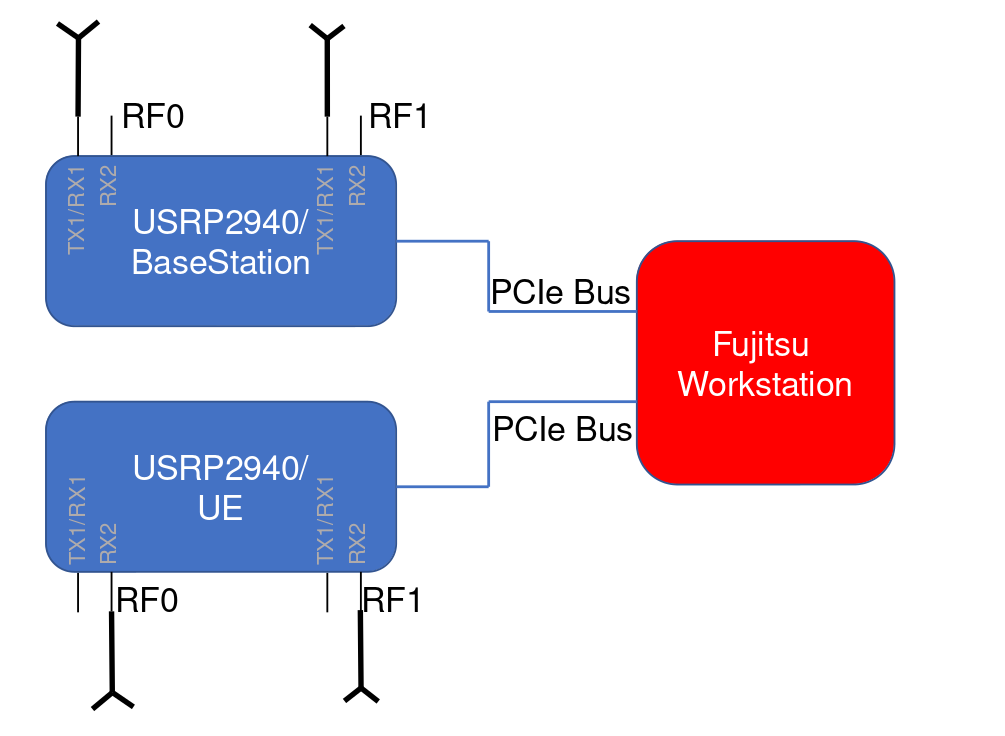
\includegraphics[width=\linewidth]{images/MIMOSetUpArrangement.png}
\caption{Overview of the LTE 2x2 MIMO HW connection setup}
\label{fig:LTEAFWHWSetup}
\end{figure}

\subsection{LTE AFW MIMO Externsion Architecture}\label{ssec:LTEAFWArch}
Placeholder

\subsection{LTE AFW Host Software}\label{ssec:LTEAFWHostSW}

\subsection{LTE AFW FPGA}\label{ssec:LTEAFWFPGA}
LTE has demanding and resource intensive processing requirements. LTE AFW aims to 

\begin{figure}[H]
\centering
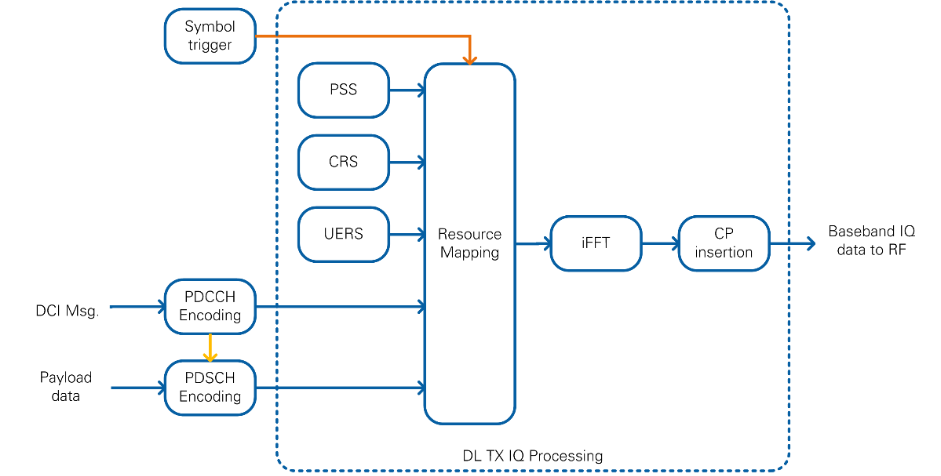
\includegraphics[width=\linewidth]{images/DLFPGATXImpl.png}
\caption{Simplified implementation of the DL TX processing block of the FPGA}
\label{fig:LTEAFWFPGADLTXProc}
\end{figure}

\begin{figure}[H]
\centering
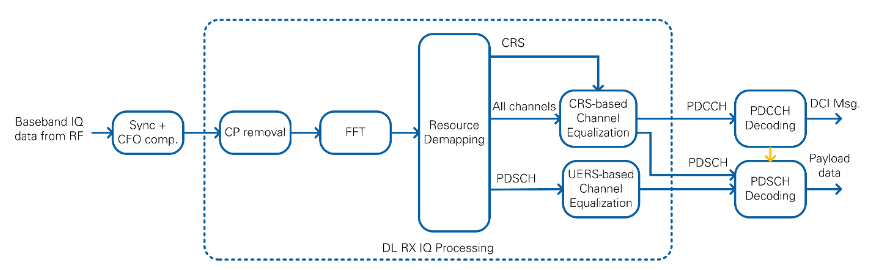
\includegraphics[width=\linewidth]{images/DLFPGARXImpl.png}
\caption{Simplified implementation of the DL RX processing block of the FPGA}
\label{fig:LTEAFWFPGADLTXProc}
\end{figure}

\section{Application Example}\label{sec:AppEx}

